% ============================================================
%  IEC 61131-3 PROGRAMMING FOR POWER SYSTEM RTACs
%  Comprehensive Study Guide
%  Covers: Overview, Data Types, ST, LD, FBD, SFC, POUs,
%          SEL RTAC Implementation, Troubleshooting, Lab
% ============================================================
\documentclass[12pt,twoside,openright]{memoir}

% ── Encoding & fonts ─────────────────────────────────────────
\usepackage[T1]{fontenc}
\usepackage[utf8]{inputenc}
\usepackage{lmodern}
\usepackage{microtype}
\usepackage{palatino}
\usepackage[scaled=0.85]{beramono}

% ── Page geometry ────────────────────────────────────────────
\usepackage[
  top=1.25in, bottom=1.25in,
  inner=1.5in, outer=1.0in,
  marginparwidth=0.8in, marginparsep=0.1in
]{geometry}

% ── Colors ───────────────────────────────────────────────────
\usepackage[dvipsnames,svgnames,x11names]{xcolor}
\definecolor{iecnavy}{HTML}{0D2137}
\definecolor{iecblue}{HTML}{1565C0}
\definecolor{ieccyan}{HTML}{0097A7}
\definecolor{iecorange}{HTML}{E65100}
\definecolor{iecgreen}{HTML}{2E7D32}
\definecolor{iecred}{HTML}{C62828}
\definecolor{iecyellow}{HTML}{F9A825}
\definecolor{rowlight}{HTML}{EFF6FF}
\definecolor{rowdark}{HTML}{DBEAFE}
\definecolor{codebg}{HTML}{0D2137}
\definecolor{codetext}{HTML}{6EE7B7}
\definecolor{frameborder}{HTML}{455A64}
\definecolor{covergray}{HTML}{ECEFF1}
\definecolor{warnbg}{HTML}{FFF3E0}
\definecolor{fieldbg}{HTML}{E8F5E9}

% ── Graphics & TikZ ──────────────────────────────────────────
\usepackage{graphicx}
\usepackage{tikz}
\usetikzlibrary{positioning,shapes.geometric,arrows.meta,decorations.pathreplacing,
                matrix,fit,backgrounds,calc,patterns,shadows.blur}
\usepackage{pgfplots}
\pgfplotsset{compat=1.18}

% ── Tables ───────────────────────────────────────────────────
\usepackage{booktabs}
\usepackage{tabularx}
\usepackage{array}
\usepackage{multirow}
\usepackage{colortbl}
\newcolumntype{L}[1]{>{\raggedright\arraybackslash}p{#1}}
\newcolumntype{C}[1]{>{\centering\arraybackslash}p{#1}}
\newcolumntype{R}[1]{>{\raggedleft\arraybackslash}p{#1}}

% ── Callout boxes (tcolorbox) ─────────────────────────────────
\usepackage[most,listings]{tcolorbox}

\newtcolorbox{keyconcept}[1][]{
  enhanced, breakable,
  colback=iecblue!8, colframe=iecblue, arc=4pt,
  fonttitle=\bfseries\sffamily\color{white}, title={Key Concept},
  attach boxed title to top left={yshift=-2mm, xshift=6mm},
  boxed title style={colback=iecblue, arc=3pt},
  #1
}

\newtcolorbox{warningbox}[1][]{
  enhanced, breakable,
  colback=warnbg, colframe=iecorange, arc=4pt,
  fonttitle=\bfseries\sffamily\color{white}, title={WARNING},
  attach boxed title to top left={yshift=-2mm, xshift=6mm},
  boxed title style={colback=iecorange, arc=3pt},
  #1
}

\newtcolorbox{fieldgotcha}[1][]{
  enhanced, breakable,
  colback=fieldbg, colframe=iecgreen, arc=4pt,
  fonttitle=\bfseries\sffamily\color{white}, title={Field Gotcha},
  attach boxed title to top left={yshift=-2mm, xshift=6mm},
  boxed title style={colback=iecgreen, arc=3pt},
  #1
}

\newtcolorbox{protip}[1][]{
  enhanced, breakable,
  colback=iecyellow!15, colframe=iecyellow!80!black, arc=4pt,
  fonttitle=\bfseries\sffamily, title={Pro Tip},
  attach boxed title to top left={yshift=-2mm, xshift=6mm},
  boxed title style={colback=iecyellow!80!black, arc=3pt},
  #1
}

% ── Code listings ─────────────────────────────────────────────
\lstdefinelanguage{ST}{
  morekeywords={VAR, VAR_INPUT, VAR_OUTPUT, VAR_IN_OUT, VAR_GLOBAL, VAR_EXTERNAL,
                RETAIN, CONSTANT, END_VAR,
                PROGRAM, END_PROGRAM, FUNCTION, END_FUNCTION,
                FUNCTION_BLOCK, END_FUNCTION_BLOCK,
                IF, THEN, ELSIF, ELSE, END_IF,
                CASE, OF, END_CASE, ELSE,
                FOR, TO, BY, DO, END_FOR,
                WHILE, DO, END_WHILE,
                REPEAT, UNTIL, END_REPEAT,
                RETURN, EXIT,
                AND, OR, NOT, XOR,
                TRUE, FALSE,
                BOOL, BYTE, WORD, DWORD, INT, DINT, UINT, UDINT,
                REAL, LREAL, TIME, DATE, STRING,
                TON, TOF, TP, CTU, CTD, CTUD},
  sensitive=false,
  morecomment=[l]{//},
  morecomment=[s]{(*}{*)},
  morestring=[b]",
}

\lstset{
  language=ST,
  basicstyle=\small\ttfamily\color{codetext},
  backgroundcolor=\color{codebg},
  keywordstyle=\color{cyan!70!white}\bfseries,
  commentstyle=\color{green!60!white}\itshape,
  stringstyle=\color{orange!80!white},
  numbers=left,
  numberstyle=\tiny\color{gray!60},
  numbersep=8pt,
  frame=single,
  rulecolor=\color{frameborder},
  breaklines=true,
  breakatwhitespace=true,
  tabsize=4,
  showstringspaces=false,
  xleftmargin=15pt,
  xrightmargin=5pt,
}

% ── Headers & footers ────────────────────────────────────────
\usepackage{fancyhdr}
\pagestyle{fancy}
\fancyhf{}
\fancyhead[LE]{\small\textcolor{iecblue}{\leftmark}}
\fancyhead[RO]{\small\textcolor{iecblue}{\rightmark}}
\fancyfoot[C]{\small\textcolor{gray}{\thepage}}
\renewcommand{\headrulewidth}{0.4pt}

% ── Hyperlinks ────────────────────────────────────────────────
\usepackage[
  colorlinks=true,
  linkcolor=iecblue,
  urlcolor=ieccyan,
  citecolor=iecgreen,
  pdftitle={IEC 61131-3 Programming for Power System RTACs},
  pdfauthor={Ricardo Barbosa},
]{hyperref}

% ── Title data ────────────────────────────────────────────────
\title{
  {\Huge\bfseries\color{iecnavy} IEC 61131-3 Programming}\\[0.5em]
  {\large\color{iecblue} for Power System RTACs}\\[0.5em]
  {\normalsize\color{gray} Structured Text, Ladder Diagram, FBD, SFC, and SEL RTAC Implementation}
}
\author{Ricardo Barbosa}
\date{2026}

% ============================================================
\begin{document}
% ============================================================

\maketitle
\thispagestyle{empty}

\vspace{2em}
\begin{center}
\resizebox{\textwidth}{!}{%
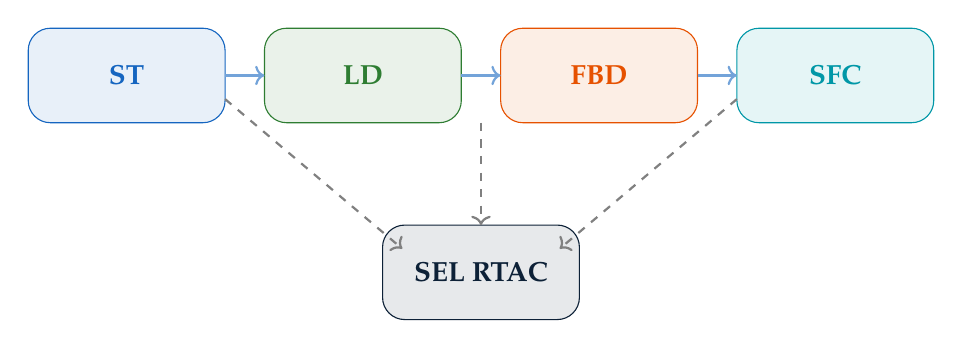
\begin{tikzpicture}
  % Cover diagram — IEC 61131-3 language icons
  \node[draw=iecblue, fill=iecblue!10, rounded corners=8pt, minimum width=2.5cm, minimum height=1.2cm]
    at (0,0) {\textbf{\color{iecblue}ST}};
  \node[draw=iecgreen, fill=iecgreen!10, rounded corners=8pt, minimum width=2.5cm, minimum height=1.2cm]
    at (3,0) {\textbf{\color{iecgreen}LD}};
  \node[draw=iecorange, fill=iecorange!10, rounded corners=8pt, minimum width=2.5cm, minimum height=1.2cm]
    at (6,0) {\textbf{\color{iecorange}FBD}};
  \node[draw=ieccyan, fill=ieccyan!10, rounded corners=8pt, minimum width=2.5cm, minimum height=1.2cm]
    at (9,0) {\textbf{\color{ieccyan}SFC}};
  \node[draw=iecnavy, fill=iecnavy!10, rounded corners=8pt, minimum width=2.5cm, minimum height=1.2cm]
    at (4.5,-2.5) {\textbf{\color{iecnavy}SEL RTAC}};
  \draw[->, thick, iecblue!60] (1.25,0) -- (1.75,0);
  \draw[->, thick, iecblue!60] (4.25,0) -- (4.75,0);
  \draw[->, thick, iecblue!60] (7.25,0) -- (7.75,0);
  \draw[->, thick, dashed, gray] (1.25,-0.3) -- (3.5,-2.2);
  \draw[->, thick, dashed, gray] (4.5,-0.6) -- (4.5,-1.9);
  \draw[->, thick, dashed, gray] (7.75,-0.3) -- (5.5,-2.2);
\end{tikzpicture}
}
\end{center}

\clearpage
\tableofcontents
\clearpage

% ============================================================
\chapter{IEC 61131-3 Overview}
% ============================================================

\section{History and Purpose}

IEC 61131-3 was first published in 1993 by the International Electrotechnical Commission Technical Committee 65 (Industrial-Process Measurement, Control, and Automation). Before its publication, every PLC vendor shipped proprietary programming software and syntax. A Siemens programmer could not read Allen-Bradley code. A Modicon programmer could not read GE code.

The standard defined five programming languages for industrial controllers, with the explicit goal of portability across vendor platforms. Portability in practice is imperfect --- every vendor implements extensions --- but the foundational knowledge transfers cleanly.

\begin{keyconcept}
\textbf{The five IEC 61131-3 languages:}
\begin{itemize}
  \item \textbf{Structured Text (ST)} --- Pascal-derived text language. The most expressive and widely used for complex logic.
  \item \textbf{Ladder Diagram (LD)} --- Graphical relay logic. Electricians can read it without software training.
  \item \textbf{Function Block Diagram (FBD)} --- Graphical data-flow. Signals flow left to right through connected blocks.
  \item \textbf{Sequential Function Chart (SFC)} --- State machine / flowchart language. Best for sequential process control.
  \item \textbf{Instruction List (IL)} --- Assembly-like. \textbf{Deprecated in the 3rd edition (2013). Do not use.}
\end{itemize}
\end{keyconcept}

\section{Third Edition (2013) Changes}

The third edition of IEC 61131-3 formally deprecated Instruction List and added object-oriented extensions to FUNCTION\_BLOCK: methods, properties, and inheritance. These OOP features are supported in CODESYS and some other modern IDEs. Support in ACSELERATOR RTAC depends on firmware version.

\section{Why It Matters for RTAC Programming}

The SEL RTAC executes IEC 61131-3 programs on a deterministic real-time kernel. Scan periods as fast as 1\,ms are supported. When you write Structured Text in ACSELERATOR RTAC, you are writing code that will execute at real-time rates alongside protocol stacks managing DNP3 communications, IEC 61850 GOOSE publishing, and relay I/O.

Platform-specific knowledge matters, but the foundational IEC 61131-3 concepts --- data types, variable scoping, POU structure, task configuration --- are identical across all compliant platforms.

% ============================================================
\chapter{Data Types and Variables}
% ============================================================

\section{Elementary Data Types}

\begin{center}
\begin{tabular}{L{2cm} C{1.5cm} L{7cm}}
\toprule
\rowcolor{iecnavy} \textcolor{white}{\textbf{Type}} & \textcolor{white}{\textbf{Size}} & \textcolor{white}{\textbf{Range / Notes}} \\
\midrule
\rowcolor{rowlight} \texttt{BOOL}   & 1 bit    & \texttt{TRUE} or \texttt{FALSE} \\
\texttt{BYTE}   & 8 bits   & 0--255. Unsigned. Bit manipulation. \\
\rowcolor{rowlight} \texttt{WORD}   & 16 bits  & 0--65535. Unsigned. \\
\texttt{DWORD}  & 32 bits  & 0--4294967295. Unsigned. \\
\rowcolor{rowlight} \texttt{INT}    & 16 bits  & $-32768$ to $+32767$. Signed. \\
\texttt{DINT}   & 32 bits  & $-2{,}147{,}483{,}648$ to $+2{,}147{,}483{,}647$. Signed. \\
\rowcolor{rowlight} \texttt{UINT}   & 16 bits  & 0--65535. Unsigned integer. \\
\texttt{REAL}   & 32 bits  & IEEE 754 single precision. $\approx$7 significant digits. \\
\rowcolor{rowlight} \texttt{LREAL}  & 64 bits  & IEEE 754 double precision. $\approx$15 significant digits. \\
\texttt{TIME}   & 32 bits  & Duration. Literal: \texttt{T\#5s}, \texttt{T\#500ms}. \\
\rowcolor{rowlight} \texttt{DATE}   & 32 bits  & Calendar date. Literal: \texttt{D\#2026-05-09}. \\
\texttt{STRING} & variable & Fixed-length. Default \texttt{STRING[80]}. \\
\bottomrule
\end{tabular}
\end{center}

\section{Variable Declaration Sections}

\begin{center}
\begin{tabular}{L{3cm} L{4.5cm} L{4cm}}
\toprule
\rowcolor{iecnavy} \textcolor{white}{\textbf{Section}} & \textcolor{white}{\textbf{Scope}} & \textcolor{white}{\textbf{Writable by caller?}} \\
\midrule
\rowcolor{rowlight}\texttt{VAR}         & Local to POU             & No --- internal only \\
\texttt{VAR\_INPUT}   & Set by caller, read by POU & Yes \\
\rowcolor{rowlight}\texttt{VAR\_OUTPUT} & Written by POU, read by caller & No \\
\texttt{VAR\_IN\_OUT} & Passed by reference (bidirectional) & Yes \\
\rowcolor{rowlight}\texttt{VAR\_GLOBAL} & Shared across all POUs   & Any POU with access \\
\texttt{VAR RETAIN}  & Survives power cycle (NVM)  & Same as \texttt{VAR} \\
\rowcolor{rowlight}\texttt{VAR CONSTANT}& Read-only within POU     & Never \\
\bottomrule
\end{tabular}
\end{center}

\begin{warningbox}
\texttt{VAR RETAIN} variables are stored in non-volatile memory. A \texttt{RETAIN} variable survives power loss and watchdog trips. Failure to mark setpoints and accumulated values as \texttt{RETAIN} means they reset to initial values after any power event --- potentially at wrong process setpoints.
\end{warningbox}

% ============================================================
\chapter{Structured Text (ST)}
% ============================================================

\section{Syntax Fundamentals}

Structured Text uses Pascal-derived syntax. Every statement ends with a semicolon. Assignment is \texttt{:=}. Comparison uses \texttt{=}, \texttt{<>}, \texttt{>}, \texttt{<}, \texttt{>=}, \texttt{<=}.

\begin{lstlisting}
(* Block comment *)
// Line comment

PROGRAM MotorInterlock
VAR
    bRunCmd      : BOOL;
    rVoltage     : REAL;
    nCount       : INT := 0;
END_VAR

bRunCmd  := TRUE;           (* Assignment operator := *)
nCount   := nCount + 1;
rVoltage := 13.8;

IF rVoltage > 14.4 THEN     (* Comparison uses = *)
    bRunCmd := FALSE;
ELSIF rVoltage < 12.0 THEN
    bRunCmd := FALSE;
ELSE
    bRunCmd := TRUE;
END_IF;
END_PROGRAM
\end{lstlisting}

\section{CASE Statement}

\begin{lstlisting}
CASE nState OF
    0: (* IDLE *)
        IF bStartCmd AND bPermissive THEN
            nState := 1;
        END_IF;
    1: (* RUNNING *)
        bMotorRun := TRUE;
        IF bStopCmd THEN
            nState    := 0;
            bMotorRun := FALSE;
        END_IF;
    ELSE
        nState := 0;  (* Catch unknown states *)
END_CASE;
\end{lstlisting}

\section{Motor Interlock Example}

The following Structured Text implements a complete motor interlock with start/stop latching, emergency stop, and fault latch logic.

\begin{lstlisting}
(* Motor Interlock — complete ST implementation *)
FUNCTION_BLOCK FB_MotorInterlock
VAR_INPUT
    bStart         : BOOL;
    bStop          : BOOL;
    bEmergencyStop : BOOL;
    bOverloadRelay : BOOL;
    bFaultReset    : BOOL;
END_VAR
VAR_OUTPUT
    bMotorRun      : BOOL;
    bFaultLamp     : BOOL;
    bReadyLamp     : BOOL;
END_VAR
VAR
    nState         : INT := 0;
    bFaultLatch    : BOOL := FALSE;
    tStartFail     : TON;
END_VAR

CASE nState OF
    0: (* IDLE *)
        bMotorRun  := FALSE;
        bReadyLamp := NOT bFaultLatch;
        tStartFail(IN := FALSE);
        IF bStart AND NOT bEmergencyStop AND NOT bFaultLatch THEN
            nState := 1;
        END_IF;

    1: (* RUNNING *)
        bMotorRun := TRUE;
        (* Start failure timer — trip if not confirmed in 5s *)
        tStartFail(IN := TRUE, PT := T#5s);
        IF tStartFail.Q THEN
            bFaultLatch := TRUE;
            nState := 2;
        END_IF;
        IF bStop OR bEmergencyStop THEN
            nState    := 0;
            bMotorRun := FALSE;
            tStartFail(IN := FALSE);
        END_IF;
        IF bOverloadRelay THEN
            bFaultLatch := TRUE;
            nState      := 2;
        END_IF;

    2: (* FAULT *)
        bMotorRun  := FALSE;
        bFaultLamp := TRUE;
        tStartFail(IN := FALSE);
        IF bFaultReset AND NOT bOverloadRelay THEN
            bFaultLatch := FALSE;
            bFaultLamp  := FALSE;
            nState      := 0;
        END_IF;
END_CASE;
END_FUNCTION_BLOCK
\end{lstlisting}

% ============================================================
\chapter{Ladder Diagram (LD)}
% ============================================================

\section{Elements and Conventions}

Ladder Diagram represents logic as horizontal rungs between two vertical power rails. The left rail is logical power (always TRUE). Each rung evaluates left to right. If the logical path is TRUE, the output coil on the right activates.

Key elements: normally open contact (--| |--), normally closed contact (--|/|--), output coil (--( )--), set coil (--(S)--), reset coil (--(R)--), TON/TOF/TP timer blocks, CTU/CTD counter blocks.

\section{Timer Function Blocks}

Three standard timer FBs are defined in IEC 61131-3:

\begin{itemize}
  \item \textbf{TON} (Timer On-Delay): Output \texttt{Q} goes TRUE after input \texttt{IN} has been TRUE for duration \texttt{PT}.
  \item \textbf{TOF} (Timer Off-Delay): Output \texttt{Q} goes TRUE immediately when \texttt{IN} goes TRUE, stays TRUE for \texttt{PT} after \texttt{IN} goes FALSE.
  \item \textbf{TP} (Pulse): Output \texttt{Q} goes TRUE for exactly \texttt{PT} when \texttt{IN} transitions TRUE.
\end{itemize}

\begin{fieldgotcha}
Each timer FB must have its own declared instance. Using the same \texttt{TON} instance for two logically separate timing functions produces incorrect behavior that is difficult to diagnose. One timer --- one instance. Always.
\end{fieldgotcha}

% ============================================================
\chapter{Function Block Diagram (FBD)}
% ============================================================

\section{Data Flow Programming}

FBD is graphical. Rectangular blocks have named inputs on the left and outputs on the right. Wires connect block outputs to block inputs. Signals flow strictly left to right. Execution order is determined by data dependency, not scan order.

Standard logic blocks: AND, OR, NOT, XOR, ADD, SUB, MUL, DIV, GT, LT, EQ. FB instances (TON, CTU, custom FBs) can also be placed as blocks in FBD.

\section{PID Control}

FBD is the preferred language for PID control loops. The \texttt{CTRL\_PID} function block takes setpoint \texttt{W} and process variable \texttt{X} as inputs and outputs control signal \texttt{Y}. The wiring topology makes the feedback loop structure immediately visible in the diagram.

% ============================================================
\chapter{Sequential Function Chart (SFC)}
% ============================================================

\section{Steps and Transitions}

SFC describes sequential behavior as a directed graph. \textbf{Steps} (rectangles) represent states. One or more steps are active at any time. An \textbf{initial step} (double border) is active at startup. \textbf{Transitions} (horizontal lines with conditions) specify when execution moves from one step to the next.

\section{Action Qualifiers}

Each action on a step has a qualifier: \textbf{N} (non-stored --- active while step active), \textbf{S} (set --- latches TRUE on step activation), \textbf{R} (reset --- resets a Set action), \textbf{P} (pulse --- one scan only on activation).

\begin{warningbox}
A Set (S) action remains active after its step deactivates. It must be explicitly Reset (R) by a downstream step. Forgetting to add the matching Reset is the most common SFC programming error.
\end{warningbox}

\section{Parallel Sequences}

A double horizontal line (AND divergence) activates multiple branches simultaneously. A double horizontal line convergence waits for all parallel branches to complete before proceeding.

% ============================================================
\chapter{POUs: Program, Function, Function Block}
% ============================================================

\section{POU Hierarchy}

\begin{center}
\resizebox{\textwidth}{!}{%
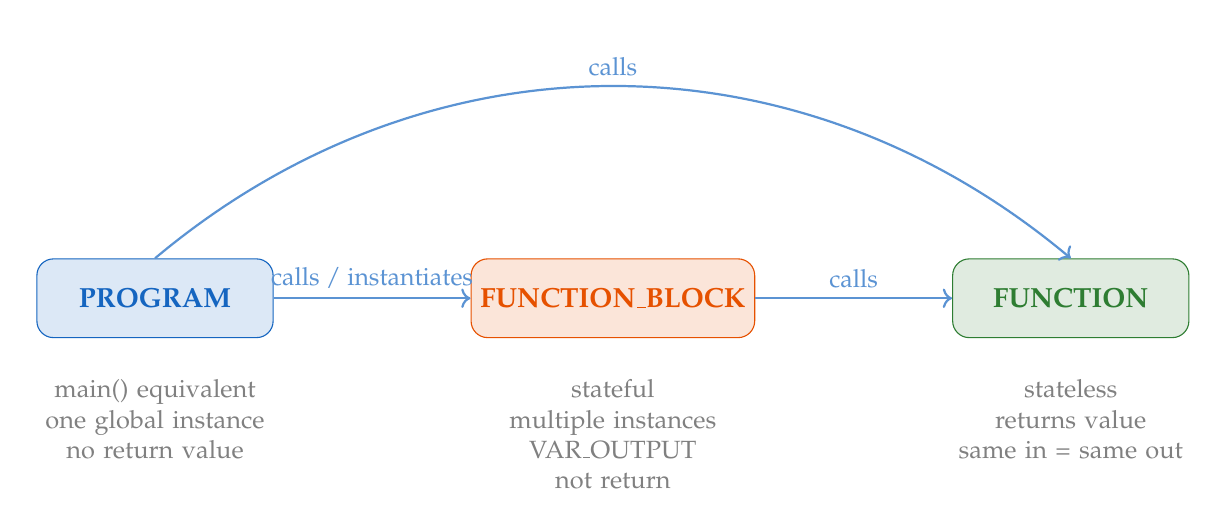
\begin{tikzpicture}[
  node distance=1.5cm and 2.5cm,
  box/.style={draw, rounded corners=6pt, minimum width=3cm, minimum height=1cm,
              text centered, font=\bfseries},
  arr/.style={->, thick, iecblue!70},
]
  % PROGRAM node
  \node[box, fill=iecblue!15, draw=iecblue] (prog)
    {\textcolor{iecblue}{PROGRAM}};
  \node[below=0.4cm of prog, font=\small, text=gray, text width=3cm, align=center] (prog-note)
    {main() equivalent\\one global instance\\no return value};

  % FUNCTION_BLOCK node
  \node[box, fill=iecorange!15, draw=iecorange, right=of prog] (fb)
    {\textcolor{iecorange}{FUNCTION\_BLOCK}};
  \node[below=0.4cm of fb, font=\small, text=gray, text width=3cm, align=center] (fb-note)
    {stateful\\multiple instances\\VAR\_OUTPUT not return};

  % FUNCTION node
  \node[box, fill=iecgreen!15, draw=iecgreen, right=of fb] (fn)
    {\textcolor{iecgreen}{FUNCTION}};
  \node[below=0.4cm of fn, font=\small, text=gray, text width=3cm, align=center] (fn-note)
    {stateless\\returns value\\same in = same out};

  % Arrows
  \draw[arr] (prog.east) -- node[above, font=\small]{calls / instantiates} (fb.west);
  \draw[arr] (fb.east)   -- node[above, font=\small]{calls} (fn.west);
  \draw[arr, bend left=40] (prog.north) to node[above, font=\small]{calls} (fn.north);
\end{tikzpicture}%
}
\end{center}

\section{FUNCTION vs. FUNCTION\_BLOCK}

The critical distinction: a \textbf{FUNCTION} is stateless --- its local variables reinitialize on every call. A \textbf{FUNCTION\_BLOCK} is stateful --- its internal variables persist between calls. To use a FUNCTION\_BLOCK, you declare a named instance; each instance has independent state.

\begin{keyconcept}
Use \texttt{FUNCTION} for pure computation (scaling, CRC, unit conversion). Use \texttt{FUNCTION\_BLOCK} for anything that needs memory between scans: timers, counters, state machines, PID controllers.
\end{keyconcept}

\section{No Recursion}

IEC 61131-3 explicitly prohibits recursive calls. A FUNCTION or FUNCTION\_BLOCK cannot call itself, directly or indirectly. The compiler detects and rejects recursive call chains. Use iteration instead.

% ============================================================
\chapter{IEC 61131-3 on the SEL RTAC}
% ============================================================

\section{ACSELERATOR RTAC IDE}

ACSELERATOR RTAC is SEL's configuration and programming IDE for the SEL-3505, SEL-3530, SEL-3555, and related RTAC family devices. The IDE integrates IEC 61131-3 programming with protocol configuration (DNP3, IEC 61850, Modbus) in a single project file.

\section{Task Configuration}

Tasks are configured with a scan period and priority. The IEC 61131-3 runtime calls each task's assigned PROGRAM at the specified interval.

\begin{center}
\begin{tabular}{C{2.5cm} L{4cm} L{5cm}}
\toprule
\rowcolor{iecnavy} \textcolor{white}{\textbf{Scan Period}} & \textcolor{white}{\textbf{Typical Use}} & \textcolor{white}{\textbf{Caution}} \\
\midrule
\rowcolor{rowlight} 1\,ms  & Fast protection, time-critical interlocks & Very tight budget \\
10\,ms & Control logic, analog processing & Common for most RTAC logic \\
\rowcolor{rowlight} 100\,ms & Status updates, protocol refresh & Comfortable budget \\
1\,s   & Logging, diagnostics & No time pressure \\
\bottomrule
\end{tabular}
\end{center}

\section{Data Mapping: Protocol to ST Variables}

The RTAC data model bridges protocol data and IEC 61131-3 variables. Protocol clients (DNP3, IEC 61850, Modbus) populate the data model. ACSELERATOR maps data model points to global variables. ST programs read and write these globals each scan.

\begin{fieldgotcha}
A global variable not mapped to a data model point always reads its initial value (0 or FALSE). If your analog reading is stuck at zero despite the remote device communicating, check the ACSELERATOR data mapping screen first.
\end{fieldgotcha}

% ============================================================
\chapter{Debugging and Troubleshooting}
% ============================================================

\section{Online Monitoring}

When connected to a live RTAC from ACSELERATOR, the watch window shows current variable values updated each scan. Variable forcing temporarily overrides program logic. \textbf{Always clear all forces before disconnecting from a production device.}

\section{Scan Time Overruns and Watchdog Trips}

If a task executes longer than its scan period, the RTAC logs a scan overrun event. Repeated overruns trigger a watchdog trip, restarting the IEC 61131-3 runtime. Non-RETAIN variables reset to initial values. RETAIN variables survive.

Common overrun causes: unbounded loops, excessive iteration counts, string operations in fast tasks, misconfigured scan period.

\section{Common RTAC IEC 61131-3 Bugs}

\begin{enumerate}
  \item State variable not initialized correctly after watchdog trip
  \item Timer instance shared between two logical uses
  \item Type mismatch without explicit conversion
  \item Global variable not mapped to data model point
  \item Scan period too aggressive for logic complexity
\end{enumerate}

% ============================================================
\chapter{Lab and Practice}
% ============================================================

\section{Free Tools}

\begin{itemize}
  \item \textbf{CODESYS} (\url{https://www.codesys.com}) --- Full IEC 61131-3 IDE with built-in soft PLC simulator. Free for development. Supports all five languages, breakpoints, watch windows.
  \item \textbf{OpenPLC Runtime} (\url{https://openplcproject.com}) --- Open-source IEC 61131-3 runtime for Linux, Windows, Raspberry Pi. Free.
  \item \textbf{BEREMIZ} (\url{https://beremiz.org}) --- Python-based open source IEC 61131-3 IDE.
\end{itemize}

\section{Suggested Exercises}

\begin{enumerate}
  \item Motor interlock in Ladder Diagram
  \item Same logic in Structured Text (CASE state machine)
  \item Encapsulate as \texttt{FB\_MotorInterlock}, instantiate three times
  \item Analog scaling \texttt{FUNCTION} with type-safe conversion
  \item Substation startup sequence in SFC (or ST CASE equivalent)
\end{enumerate}

\begin{protip}
Complete all exercises in CODESYS with simulation before touching ACSELERATOR RTAC. The logic validation work is identical in both environments. CODESYS gives you breakpoints.
\end{protip}

% ============================================================
\appendix
\chapter{Quick Reference}
% ============================================================

\section{ST Operators Summary}

\begin{center}
\begin{tabular}{L{3cm} L{3cm} L{5cm}}
\toprule
\rowcolor{iecnavy} \textcolor{white}{\textbf{Category}} & \textcolor{white}{\textbf{Operators}} & \textcolor{white}{\textbf{Notes}} \\
\midrule
\rowcolor{rowlight} Assignment    & \texttt{:=}                  & Not \texttt{=} \\
Arithmetic    & \texttt{+ - * / MOD}         & Standard math \\
\rowcolor{rowlight} Comparison    & \texttt{= <> > < >= <=}      & Returns \texttt{BOOL} \\
Logical       & \texttt{AND OR NOT XOR}      & On \texttt{BOOL} operands \\
\rowcolor{rowlight} Bitwise       & \texttt{AND OR NOT XOR}      & On \texttt{BYTE/WORD/DWORD} \\
Shift         & \texttt{SHL(x,n) SHR(x,n)}  & Shift left/right by $n$ bits \\
\bottomrule
\end{tabular}
\end{center}

\section{Professional Certification Context}

No individual exam-based credential currently exists specifically for IEC 61131-3. Practitioners in industrial automation who work with IEC 61131-3 typically pursue:

\begin{itemize}
\item \textbf{ISA CCST} (Certified Control Systems Technician) --- covers industrial communications protocols, PID control, SCADA integration, and field instrumentation. Levels I, II, and III based on experience. See isa.org/certification/ccst.
\item \textbf{ISA CAP} (Certified Automation Professional) --- broader engineering credential covering process control, automation systems, and integration. Requires engineering background. See isa.org/certification/cap.
\item \textbf{Vendor-Specific Context}:
  \begin{itemize}
  \item For Modbus: Inductive Automation Core/Gold certification tests Modbus connectivity in Ignition context.
  \item For DNP3: Triangle Microworks and SEL University offer training (PDHs, not credentials).
  \item For OPC UA: MatrikonOPC OPCSI is a vendor-sponsored credential for OPC systems integrators.
  \item For IEC 61131-3: Vendor-specific certs (Rockwell, Siemens, Beckhoff) test platform-specific implementations. SEL University APP RTAC ADV-1 covers IEC 61131-3 in RTAC context.
  \item For RTAC: SEL University APP RTAC course awards PDHs. No formal credential exam.
  \end{itemize}
\end{itemize}

\end{document}
